\documentclass[11pt]{article}
\usepackage{amsmath}
\usepackage{amssymb}
\usepackage{amsthm}
\usepackage{amscd}
\usepackage{amsfonts}
\usepackage{graphicx}%
\usepackage{fancyhdr}
\usepackage{color}
\usepackage{cite}

%\usepackage[T1]{fontenc}
\usepackage[utf8]{inputenc}
\usepackage{authblk}
\usepackage{physics}
\usepackage{float}
\usepackage{caption}
\usepackage{subcaption}
\newcommand{\expv}[1]{\ensuremath{\mathbb{E}[ #1]}}
\newcommand{\xs}[2]{\ensuremath{\Sigma_{#1}^{(#2)}}}
\newcommand{\intO}{\ensuremath{\int\limits_{4\pi}}}
\newcommand{\intz}{\ensuremath{\int\limits_0^1}}
\newcommand{\intf}{\ensuremath{\int\limits_{-\infty}^\infty}}
\newcommand{\intzf}{\ensuremath{\int\limits_{0}^\infty}}
\newcommand{\LargerCdot}{\raisebox{-0.25ex}{\scalebox{1.2}{$\cdot$}}}

\textwidth6.6in
\textheight9in


\setlength{\topmargin}{0.3in} \addtolength{\topmargin}{-\headheight}
\addtolength{\topmargin}{-\headsep}

\setlength{\oddsidemargin}{0in}

\oddsidemargin  0.0in \evensidemargin 0.0in \parindent0em

%\pagestyle{fancy}\lhead{MATH 579 (UQ for PDEs)} \rhead{02/24/2014}
%\chead{Project Proposal} \lfoot{} \rfoot{\bf \thepage} \cfoot{}


\begin{document}

\title{Sparse Stochastic Collocation \\Uncertainty Quantification \\for Multigroup Diffusion}

\author[]{Paul Talbot\thanks{talbotp@unm.edu}}
\affil[]{Department of Chemical and Nuclear Engineering\\University of New Mexico}
%\date{}
\renewcommand\Authands{ and }
\maketitle
\newpage
\section{Introduction}
There have been many recent advances in uncertainty quantification in numerical models for computational physics \cite{SCLagrange}.  In this document, we present ongoing work to demonstrate the efficiency of sparse-grid stochastic collocation \cite{sparseSC} in comparison with analog Monte Carlo for uncertainty quantification.

\subsection{General Problem}
Uncertainty quantification can be applied to many computational models.  The physical system we consider in this work is a two-dimensional quarter-core nuclear reactor. We apply reflective symmetry on the left and bottom boundaries to solve a full two-dimensional core, consisting of 5 materials distributed in 121 regions.  Figure \ref{geom} shows the geometry of the core.  The mathematical problem we solve addresses the neutronics of the core, in particular the two-group neutron diffusion criticality approximation.

\subsection{Deterministic Problem}
The neutron flux is approximated by the coupled system of elliptic PDEs
\begin{equation}
-\grad\cdot\qty( D_1(\bar x)\grad\phi_1(\bar x))+\qty(\xs{a}{1}(\bar x)+\xs{s}{1\to2}(\bar x))\phi_1(\bar x) = \frac{1}{k(\phi)}\sum_{g'=1}^2\nu_{g'}\xs{f}{g'}(\bar x)\phi_{g'}(\bar x),
\end{equation}
\begin{equation}
-\grad \cdot\qty(D_2(\bar x)\grad \phi_2(\bar x))+\xs{a}{2}(\bar x)\phi_2(\bar x) = \xs{s}{1\to 2}(\bar x)\phi_1(\bar x),
\end{equation}
where we use the following parametric coefficients: the absorption cross section $\Sigma_{g,a}=\Sigma_{g,c}+\Sigma_{g,f}$; the capture and fission cross sections $\Sigma_{g,c}$ and $\Sigma_{g,f}$; the diffusion coefficient $D_g$ which depends on the scattering cross section of the medium; and the fission multiplication factor $\nu_g$, the ratio of new neutrons per fission-producing neutron.  The solution to this PDE is the neutron scalar flux $\phi_g(\bar x)$.  We apply no-traction conditions on the vacuum boundaries and zero-derivative current on the reflecting boundaries for both energy groups:
 \begin{equation}
\frac{\phi_g}{4}-\frac{D_g}{2}\eval{\pdv{\phi_g}{x_1}}_{\partial \Omega_\text{top}}=0,\hspace{5pt} g=1,2,
\end{equation}
\begin{equation}
\frac{\phi_g}{4}-\frac{D_g}{2}\eval{\pdv{\phi_g}{x_2}}_{\partial \Omega_\text{right}}=0,\hspace{5pt} g=1,2,
\end{equation}
\begin{equation}
-D_g\eval{\pdv{\phi_g}{x_1}}_{\partial \Omega_\text{bottom}}=0,\hspace{5pt} g=1,2,
\end{equation}
\begin{equation}
-D_g\eval{\pdv{\phi_g}{x_2}}_{\partial \Omega_\text{left}}=0,\hspace{5pt} g=1,2.
\end{equation}
\\
The criticality eigenvalue and quantity of interest $k(\phi)$ is given by
\begin{equation}
k(\phi)=\sum_{g=1}^2\iint\limits_D\frac{\nu\xs{f}{g}\phi_g(\bar x)}{\qty(-\nabla\cdot D_g\nabla+\Sigma_r^{(g)})\phi_g(\bar x)}~d\bar x.
\end{equation}
We address solving $\phi_1,\phi_2,$ and $k$ nonlinearly and simultaneously.  
The material properties are shown in Table \ref{tab:coremats}, and the domain $\Omega=[0,200\text{ cm}]^2$.  The reference flux solutions are plotted in Fig. \ref{benchflux}, and for the reference problem $k$=1.00007605445.
\begin{figure}[H]
\centering
  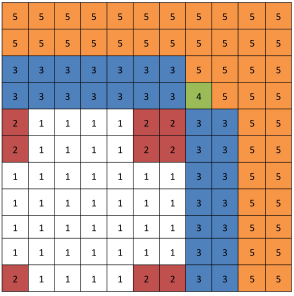
\includegraphics[width=0.4\linewidth]{core}
  \caption{Core Geometry}
  \label{geom}
\end{figure}
\begin{table}[h]
\centering
\begin{tabular}{c c | c c c c}
Region & Group & $D_g$ & $\Sigma_{a,g}$ & $\nu\Sigma_{f,g}$ & $\Sigma_s^{1,2}$ \\ \hline
1 & 1 & 1.255 & 8.252e-3 & 4.602e-3 & 2.533e-2 \\
 & 2 & 2.11e-1 & 1.003e-1 & 1.091e-1 & \\ \hline
2 & 1 & 1.268 & 7.181e-3 & 4.609e-3 & 2.767e-2 \\
 & 2 & 1.902e-1 & 7.047e-2 & 8.675e-2 & \\ \hline
3 & 1 & 1.259 & 8.002e-3 & 4.663e-3 & 2.617e-2 \\
 & 2 & 2.091e-1 & 8.344e-2 & 1.021e-1 & \\ \hline
4 & 1 & 1.259 & 8.002e-3 & 4.663e-3 & 2.617e-2 \\
 & 2 & 2.091e-1 & 7.3324e-2 & 1.021e-1 & \\ \hline
5 & 1 & 1.257 & 6.034e-4 & 0 & 4.754e-2 \\
 & 2 & 1.592e-1 & 1.911e-2 & 0 & 
\end{tabular}
\caption{Reference Material Properties for Benchmark Core}
\label{tab:coremats}
\end{table}
\begin{figure}[H]
\centering
  \begin{subfigure}[b]{0.45 \textwidth}
   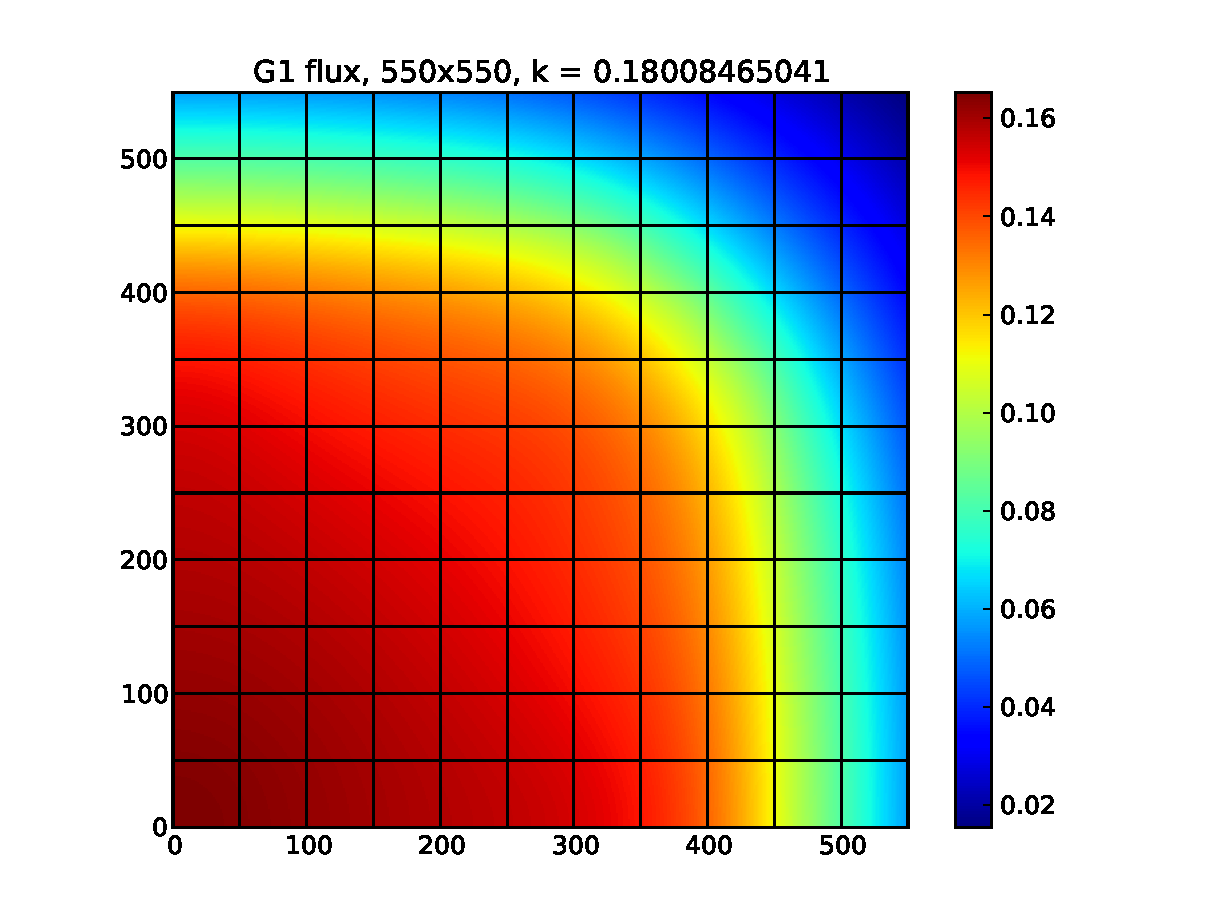
\includegraphics[width=\textwidth]{g1_50_flux}
   \caption{$\phi$, Group 1}
   \label{g1}
  \end{subfigure}
  \begin{subfigure}[b]{0.45 \textwidth}
   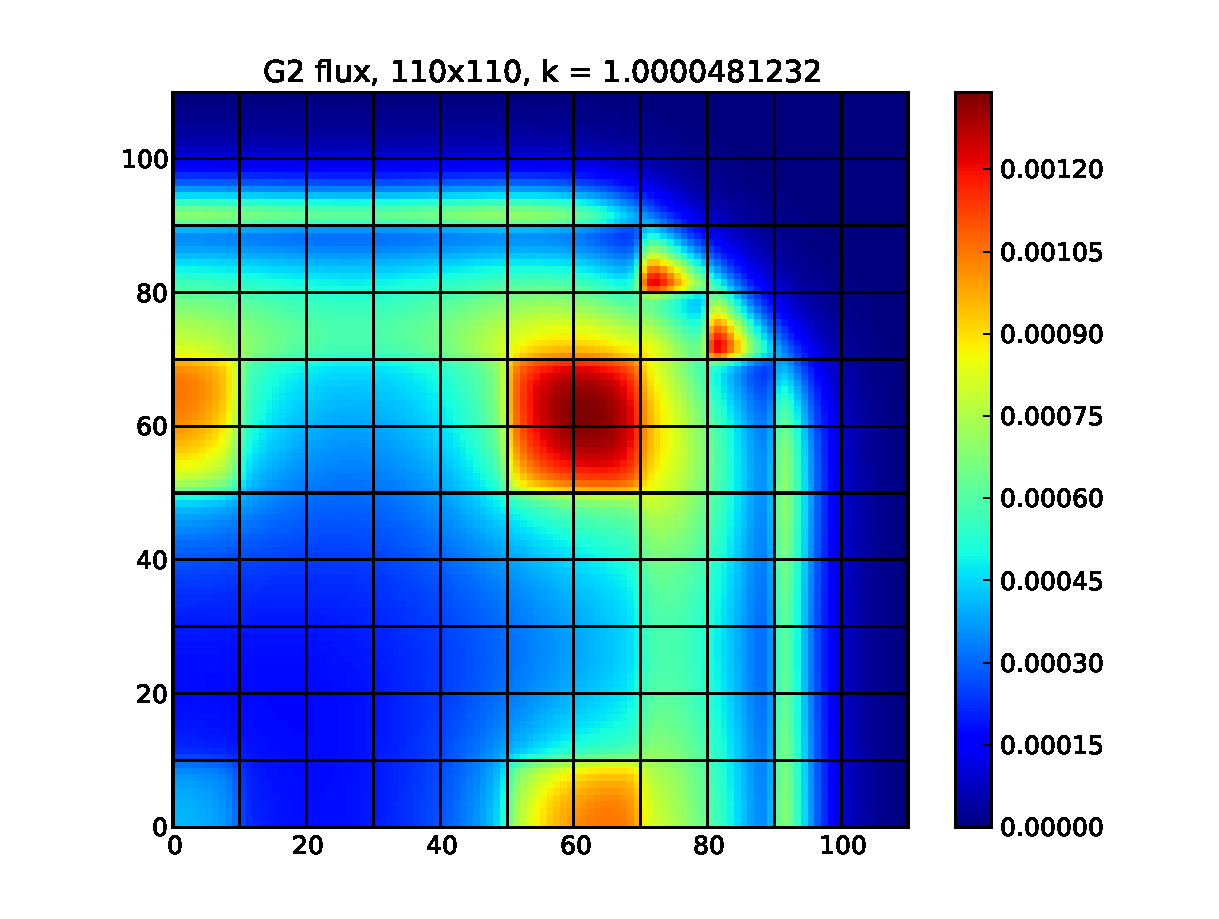
\includegraphics[width=\textwidth]{g2_50_flux}
   \caption{$\phi$, Group 2}
   \label{g2}
  \end{subfigure}
  \caption{Reference Flux Profiles}
  \label{benchflux}
\end{figure}

\subsection{Stochastic Problem}
All the macroscopic cross sections, along with the neutron multiplication factor $\nu$ and diffusion coefficient $D$, are potential sources of uncertainty for each energy group.  For this study, we consider uncertainty in several of the low-energy macroscopic cross sections as well as the reflecting material diffusion coefficient.  We introduce uniformly-distributed uncertainty from 10\% below the reference value to 10\% higher than the reference value.  The combination of these uncertain distributions make up the uncertainty space $\Gamma\subset\mathbb{R}^N,$ where $N$ is the number of uncertain parameters.  We also consider these cross section uncertainties to be independent; that is, for a vector of uncertain parameters $Y=[Y_1,\cdots,Y_N]$, the joint probability distribution $\rho(Y)$ is given by the product of individual probability distributions $\rho_n(Y_n)$, $1\leq n\leq N$,
\begin{equation}
\rho(Y) = \prod_{n=1}^N \rho_n(Y_n).
\end{equation}



\section{Motivation}
One of the most common currently-employed tools for uncertainty quantification is Monte Carlo sampling.  Each history involves randomly sampling from $\Gamma$ and solving the PDE system for a single realization.
The convergence rate of Monte Carlo to the expectation value of the analytic solution follows $\epsilon=c\ M^{-1/2}$, where $\epsilon$ is the error, $c$ is a constant independent of $M$, and $M$ is the number of histories.  While Monte Carlo is a stable method, often $M$ must be very large to converge on an appropriate magnitude of error.  This translates to large costs, especially as difficulty in solving the PDEs increases.\\

Our goal is to explore sparse-grid stochastic collocation methods as an informed approach to significantly reduce error for the same computational cost as analog Monte Carlo. 

\section{Methods}
\subsection{Deterministic Space}
We solve our system of equations by imposing a mesh grid on the physical domain using the finite volume method, a local and global particle-conserving method similar to piecewise constant finite elements.  We solve the system of equations nonlinearly with the criticality eigenvalue, using Jacobian-free Newton-Krylov methods.  In particular we use the GMRES algorithm in the \texttt{trilinos} solver package from Sandia National Laboratory \cite{Trilinos-Overview}.  

\subsection{Stochastic Space}
Our primary interest in this study is evaluating the practicality of using stochastic collocation on sparse grids \cite{sparse1}\cite{sparse2}\cite{sparseSC} to quantify uncertainty in diffusion problems.  As a benchmark we compare isotropic sparse grid stochastic collocation to analog Monte Carlo uncertainty quantification.  We use a high-resolution solution for the expected value of $k$ in stochastic space as a reference solution, and compare Monte Carlo and stochastic collocation solutions to the reference as a function of the number of transport solves. \\

In stochastic solves, we treat the deterministic transport solver non-intrusively as a functional of the uncertain input parameters.  To avoid confusion in labels, we will represent $k(Y)$ by a more generic $u(Y)$.

\subsubsection{Monte Carlo}
In Monte Carlo uncertainty quantification, the uncertain vector $Y$ is randomly sampled $M$ times, and moments are derived from the solution realizations.  For example, 
\begin{equation}
\expv{u(Y)} = \int_\Gamma u(Y) \rho(Y) dY\approx \frac{1}{M}\sum_{m=1}^M u(Y_m),
\end{equation}
\begin{equation}
\expv{u(Y)^2} = \int_\Gamma u(Y)^2 \rho(Y) dY\approx \frac{1}{M}\sum_{m=1}^M u(Y_m)^2,
\end{equation}
where each $Y_m$ is a single realization randomly sampled from the domain of $Y$.

\subsubsection{Stochastic Collocation}
In stochastic collocation for sparse grids, we approximate $u(Y)$ as the sum of $u$ evaluated at $\eta$ collocated points multiplied by multidimensional Lagrangian polynomials.  We make use of the quadrature index $k$, not to be confused with the criticality factor $k(Y)$ (represented here in stochastic form by $u(Y)$).
\begin{equation}\label{approx}
u(Y)\approx u_{h,\eta,\Lambda(L)}(Y)=\sum_{k=0}^\eta u(Y^{(k)})\mathcal{L}_k(Y),
\end{equation}
\begin{equation}
\mathcal{L}_k(Y)=\prod_{n=1}^N \mathcal{L}_{k_n}(Y_n),
\end{equation}
\begin{equation}
\mathcal{L}_{k_n}(Y_n)=\prod_{j=1}^i \frac{Y_n-Y_n^{(i)}}{Y_n^{(k_n)}-Y_n^{(i)}},
\end{equation}
\begin{equation}
\expv{u(Y)}\approx\expv{u_h(Y)}=\sum_{k=1}^\eta w_k ~u_h\qty(Y^{(k)}),
\end{equation}
where $u_h(Y)$ is the spatially-discretized PDE solution, and $Y^{(k)}=[Y^{(k_1)},\cdots,Y^{(k_N)}]$ are realizations of $Y$ similar to $Y_m$ in Monte Carlo but chosen at quadrature points $Y^{(k)}$ with corresponding weights $w_k$.  For this study, uniformly-distributed uncertain parameters suggest Gauss-Legendre quadrature to obtain collocation points and weights.  The necessary quadrature points are obtained based on polynomial expansion orders from an index set $\Lambda(L)$.  \\

The index set $\Lambda(L)$ provides the basis for most of the polynomial representation, including determining the quadrature set to evaluate the sum in Eq. \ref{approx}.  For example, for a single uncertain parameter ($N=1$) and a fourth-order polynomial approximation ($L=4$), $\Lambda$ includes all polynomial orders from 0 to 4, $\qty(\Lambda=[0,1,2,3,4])$.  Each index point $p\in\Lambda$ corresponds to a polynomial expansion moment of order $i$.\\

In the multivariate case, there are several methods to determine what index set to use.
In the most naive case, $\Lambda(L)$ is a tensor product of polynomial expansion orders,
\begin{equation}
\Lambda_\text{TP}(L)=\Big\{\bar p=[p_1,...,p_N]: \max_{1\leq n\leq N}p_n\leq L \Big\},\hspace{10pt}|\Lambda_\text{TP}(L)|=(L+1)^2.
\end{equation}
For example, for $N=2$ and $L=4$, the index set $\Lambda_\text{TP}(L)$ includes all combinations of the expansion orders $[0,1,2,3,4]\otimes[0,1,2,3,4]$ for a total of 25 polynomial expansion indices.  The collection of expansion points in this example index set is shown in Fig. \ref{TP}.  \\

Other index sets with less cardinality can be employed to reduce the number of collocation points.  Two in particular are the ``total degree'' set (see Fig. \ref{TD}), which is ideal for quantities that are analytic in stochastic space,
\begin{equation}
\Lambda_\text{TD}(L)=\Big\{\bar p=[p_1,...,p_N]:\sum_{n=1}^N p_n \leq L \Big\},\hspace{10pt}|\Lambda_\text{TD}(L)|={L+N\choose N},
\end{equation}
and the ``hyberbolic cross'' index set (see Fig. \ref{HC}), for quantities that have limited smoothness in stochastic space,
\begin{equation}
\Lambda_\text{HC}(L)=\Big\{\bar p=[p_1,...,p_N]:\prod_{n=1}^N p_n+1 \leq L+1 \Big\},\hspace{10pt}|\Lambda_\text{HC}(L)|\leq (L+1)(1+\log(L+1))^{N-1}.
\end{equation}
Figure \ref{indexsets} shows each of these index sets for $N=2,L=4$.  The savings of total degree and hyperbolic cross help fight the curse of dimensionality present in tensor product. 
\begin{figure}[H]
\centering
  \begin{subfigure}[b]{0.32 \textwidth}
   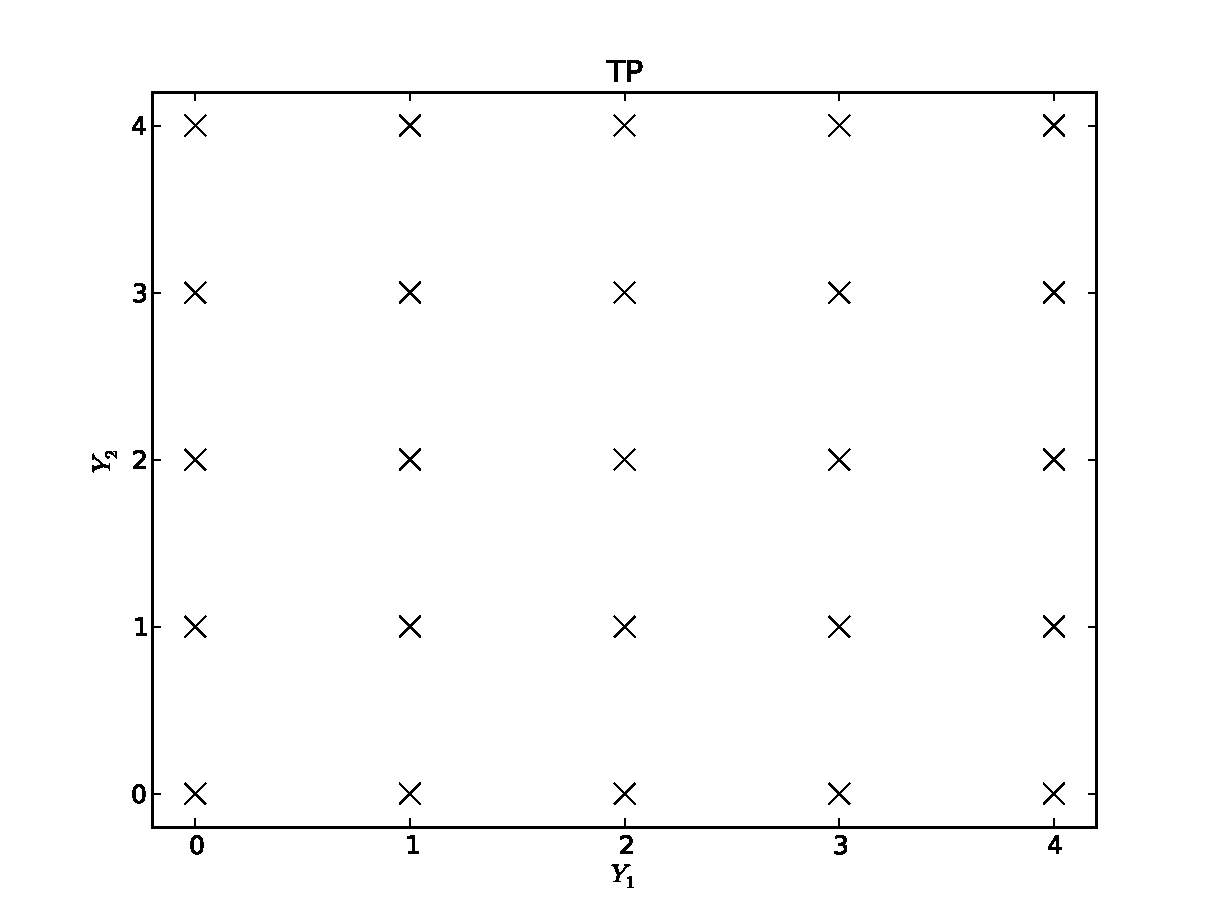
\includegraphics[width=\textwidth]{TP}
   \caption{Tensor Product}
   \label{TP}
  \end{subfigure}
  \begin{subfigure}[b]{0.32 \textwidth}
   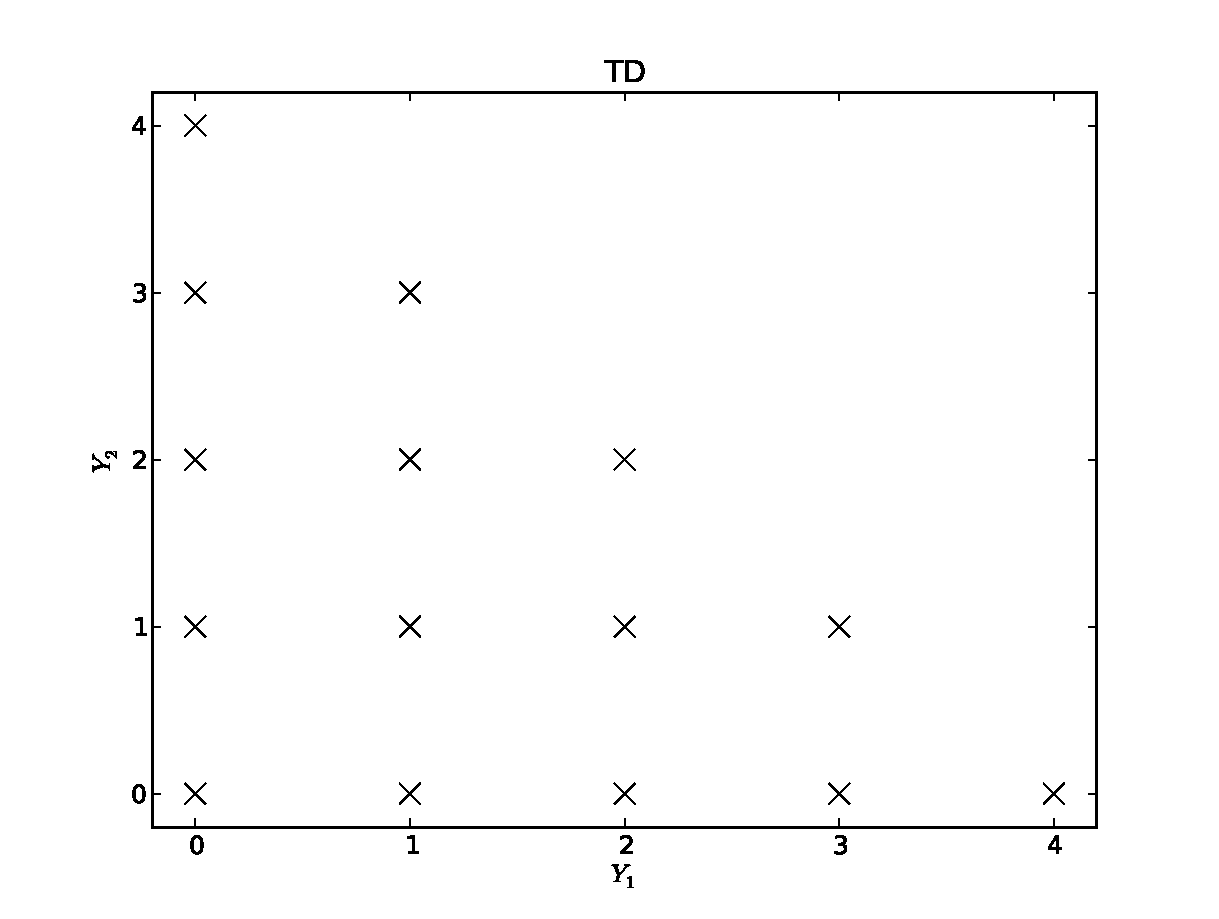
\includegraphics[width=\textwidth]{TD}
   \caption{Total Degree}
   \label{TD}
  \end{subfigure}
  \begin{subfigure}[b]{0.32 \textwidth}
   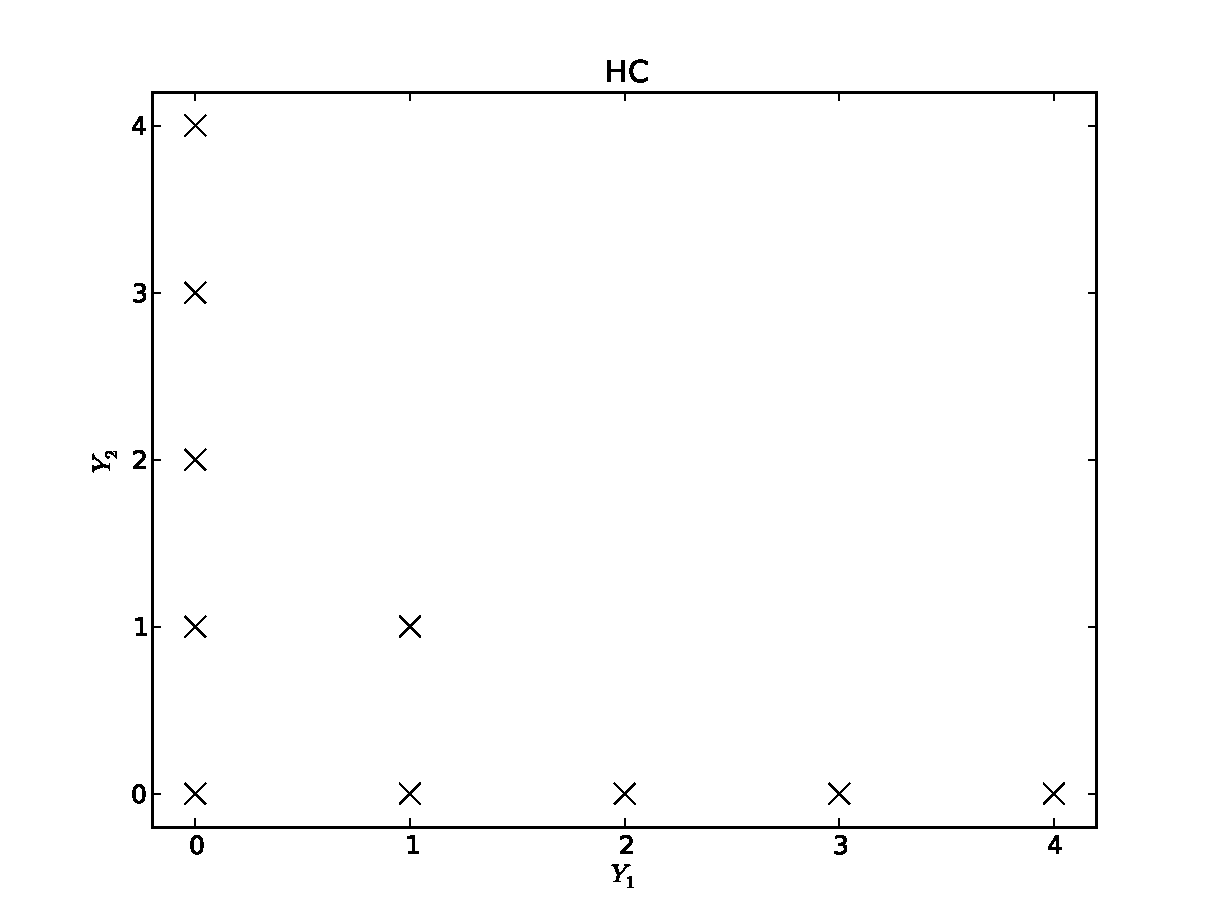
\includegraphics[width=\textwidth]{HC}
   \caption{Hyperbolic Cross}
   \label{HC}
  \end{subfigure}
  \caption{Index Set Examples: $N=2,L=4$}
  \label{indexsets}
\end{figure}
%\begin{figure}[H]
%\centering
%  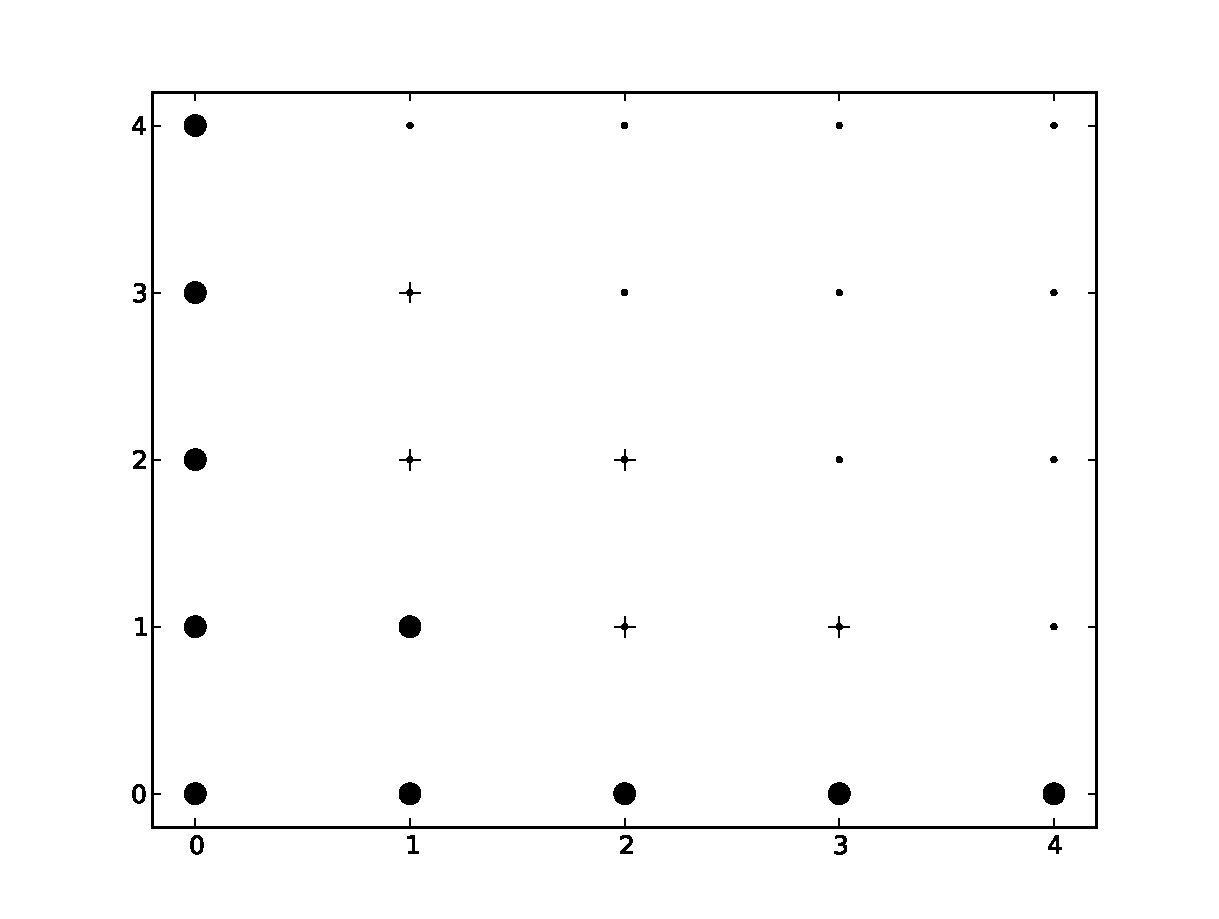
\includegraphics[width=0.5\linewidth]{indexsets}
%  \caption{Index Sets ($\cdot$ TP, + TD, $\bullet$ HC) }
%  \label{indexsets}
%\end{figure}


The collocation points used in the Lagrange polynomial expansion are obtained based on the index set chosen.  To uniquely specify an isotropic Smolyak-like sparse grid, it is necessary to select the number of uncertain variables $N$, the desired expansion order $L$, the index set $\Lambda(L)$, the quadrature rule $p(i)$, and the quadrature points-and-weights generating function for one-dimensional quadratures.
This provides the isotropic sparse grid approximation
\begin{equation}
k(Y)\approx\mathcal{S}_{N,\Lambda(L)}[k](Y)=\sum_{\boldsymbol{i}\in\Lambda(L)}c(\boldsymbol{i})\bigotimes_{n=1}^N\mathcal{U}_{n,p(i_n)}[u](Y),
\end{equation}
\begin{equation}
c(\boldsymbol{i})=\sum_{\substack{\boldsymbol{j}=\{0,1\}^N,\\ \boldsymbol{i}+\boldsymbol{j}\in\Lambda(L)}}(-1)^{|\boldsymbol{j}|_1},
\end{equation}
\begin{align}
\bigotimes_{n=1}^N\mathcal{U}_{n,p(i_n)}[u](Y)&\equiv\sum_{k_1=0}^{p(i_1)}\cdots\sum_{k_N=0}^{p(i_N)}u_h\qty(Y^{(k_1)},\cdots,Y^{(k_N)})\prod_{n=1}^N \mathcal{L}_{k_n}(Y_n),\\
  &=\sum_{k}^{p(\vec i)}u_h\qty(Y^{(k)})\mathcal{L}_k(Y),
\end{align}
where $p(i)$ is the ``quadrature rule'' used to obtain the number of quadrature points for a given expansion order.  While this can be chosen arbitrarily, it is common to select $p(i)=i$ for Gauss quadrature and $p(i)=2^i$ for Clenshaw-Curtis quadrature.
The sparse grid quadrature is obtained through the tensor product of smaller quadratures, which has less cardinality than the full tensor quadrature.  The savings in collocation points are demonstrated in Figure \ref{collsets} for two identically distributed uniform variables, each on [-1,1].  The reduction in collocation points grows with the number of input parameters $N$ and the expansion order $L$.  \\

For comparison, we show the number of index points for two input spaces of dimensionality $N$ and several expansion levels $L$ for all three index sets, as well as the number of collocation points for total degree and hyperbolic cross rules in Table \ref{compIS}.  We note that accuracy cannot be directly drawn from polynomial expansions; as shown in Section \ref{results}, for this problem the same number of collocation points results in a similar magnitude error in both total degree and hyperbolic cross.  This implies, for this problem, that a much lower-order polynomial expansion constructed using the total degree rule is comparable in error to a larger-order polynomial expansion constructed using the hyperbolic cross rule.
\begin{figure}[H]
\centering
  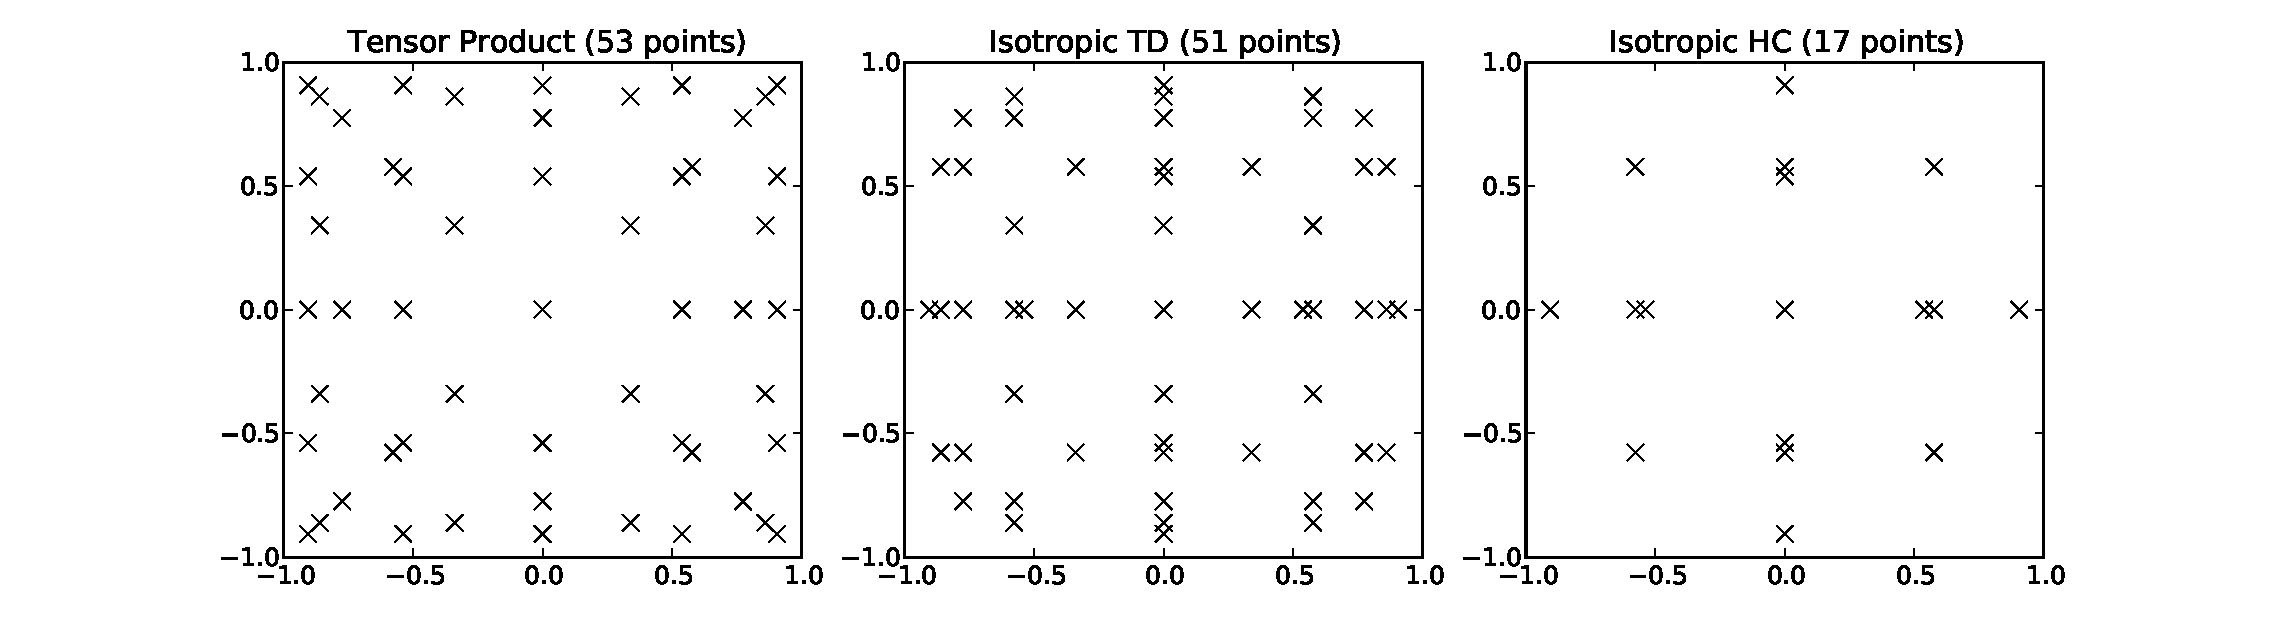
\includegraphics[width=\linewidth]{sparse_plot}
  \caption{Sparse Grids, $N=2,L=4,p(i)=i$, Legendre points}
  \label{collsets}
\end{figure}
\begin{table}
\centering
\begin{tabular}{c|c|c|c c|c c}
$N$ & $L$ & TP & \multicolumn{2}{|c|}{TD} & \multicolumn{2}{|c}{HC} \\ 
$N$ & $L$ & $\qty|\Lambda(L)|$ & $\qty|\Lambda(L)|$ & $\eta$ & $\qty|\Lambda(L)|$ & $\eta$\\ \hline
3 & 4 & 125    & 35    & 165   & 16 & 31\\
 & 8   & 729    & 165  & 2,097  & 44 & 153\\
 & 16 & 4,913  & 969   & 41,857 & 113 & 513\\
 & 32 & 35,737 & 6,545 & 1,089,713 & 309 & 2,181\\ \hline
5 & 2 & 293 & 21 & 61 & 11 & 11\\
 & 4 & 3,125 & 126 & 781 & 31 & 71\\
 & 8 & 59,049 & 1,287 & 28,553 & 111 & 481 
\end{tabular}
\caption{Index Set and Collocation Size Comparison}
\label{compIS}
\end{table}
While the hyberbolic cross collocation points are significantly more sparse than the total degree collocation points, we note that the increased number of polynomial expansion moments in total degree make it much more accurate for the same total polynomial expansion level $L$.  The results of this work demonstrate that for this problem, the same number of collocation points using either total degree or hyperbolic cross results in a similar magnitude of error.

\subsubsection{Anisotropic Sparse Grid}
One disadvantage of sparse grids as defined above is that it treats all dimensions of uncertainty space equally.  In many cases, however, the sensitivity of the stochastic solution to one dimension is less than another.  For example, we heuristically expect the sensitivity of the $k$-eigenvalue to the reflecting material (material 5) diffusion coefficient to be much less than the sensitivity to the fission cross section in the main fissile material (material 1).  \\

We can leverage the varying sensitivity by introducing importance parameters $\vec\alpha=[\alpha_1,\cdots,\alpha_N]$ that parametrize the sensitivity of the stochastic solution to each dimension.  Using the one-norm
\begin{equation}
\qty|\vec\alpha|_1\equiv\frac{1}{N}\sum_{n=1}^N \alpha_n,
\end{equation}
these weight parameters adjust the index set rules $\Lambda(L)$ for total degree and hyperbolic cross as
\begin{equation}
\tilde\Lambda_\text{TD}(L)=\Big\{\bar p=[p_1,...,p_N]:\sum_{n=1}^N \alpha_n p_n \leq \qty|\vec\alpha|_1 L \Big\},
\end{equation}
\begin{equation}
\tilde\Lambda_\text{HC}(L)=\Big\{\bar p=[p_1,...,p_N]:\prod_{n=1}^N \qty(p_n+1)^{\alpha_n} \leq \qty(L+1)^{\qty|\vec\alpha|_1} \Big\}.
\end{equation}
In this formulation, greater values of $\alpha_n$ result in less quadrature points for uncertain input $Y_n$.  Smaller values of $\alpha_n$ are assigned to more sensitive dimensions to prioritize collocation points.


\section{Results}\label{results}
\subsection{Deterministic Convergence}
In Figs. \ref{spatialphi}-\ref{spatialk} we demonstrate the physical convergence of the deterministic PDE solver as we refine the spatial mesh grid.  Both fluxes as well as the $k$-eigenvalue converge between first and second order.  The finite volume method is second order, but the overall convergence order is reduced by first-order boundary condition treatments.  In all cases, reducing the size of $h=\Delta x=\Delta y$ decreases the error to a fine solution.  The reference solution is one level of refinement finer than the finest point shown.   The flux error is calculated by considering the maximum error among several pointwise flux values, while $k$ error is the global value for each refinement.
\begin{figure}[H]
\centering
  \begin{subfigure}[b]{0.45 \textwidth}
   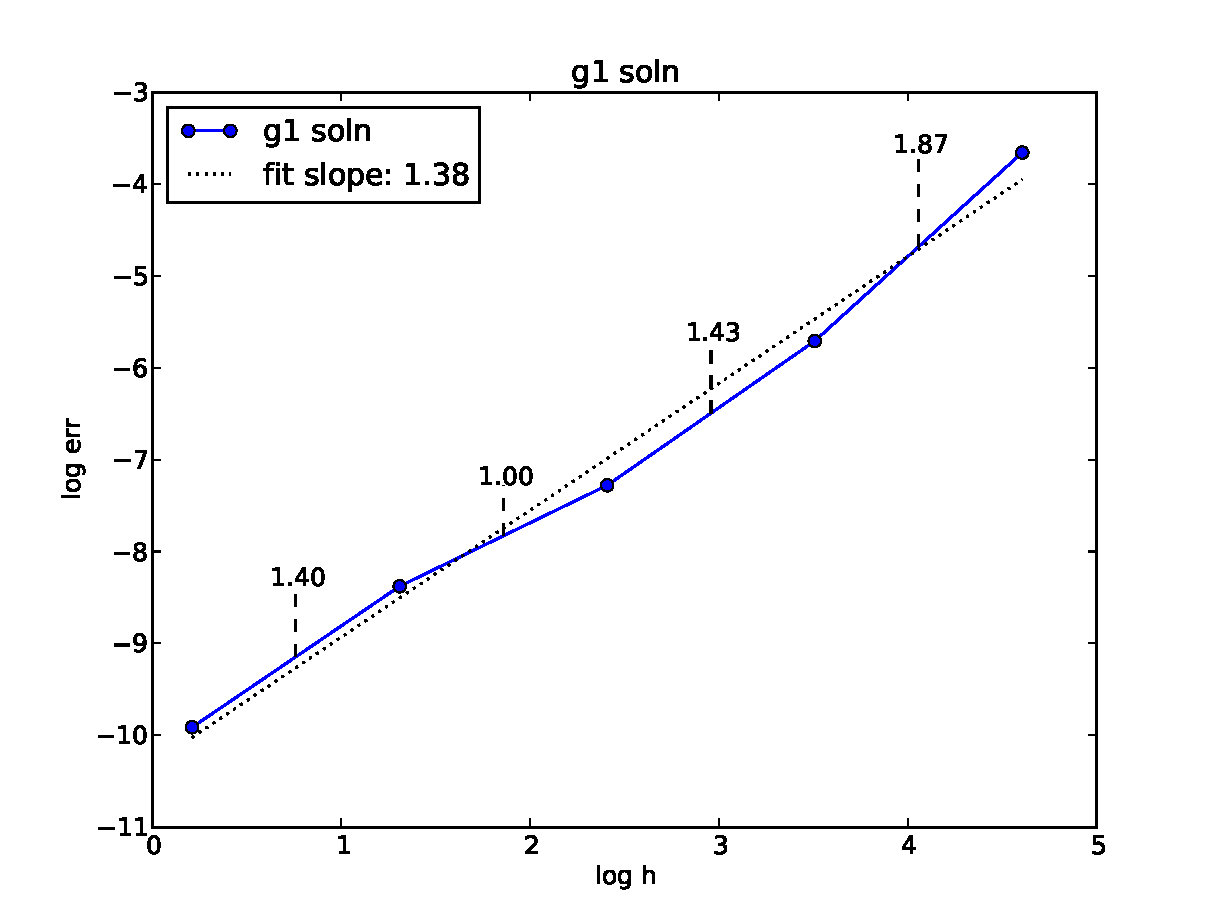
\includegraphics[width=\textwidth]{g1}
   \caption{$\phi$, Group 1}
   \label{g1}
  \end{subfigure}
  \begin{subfigure}[b]{0.45 \textwidth}
   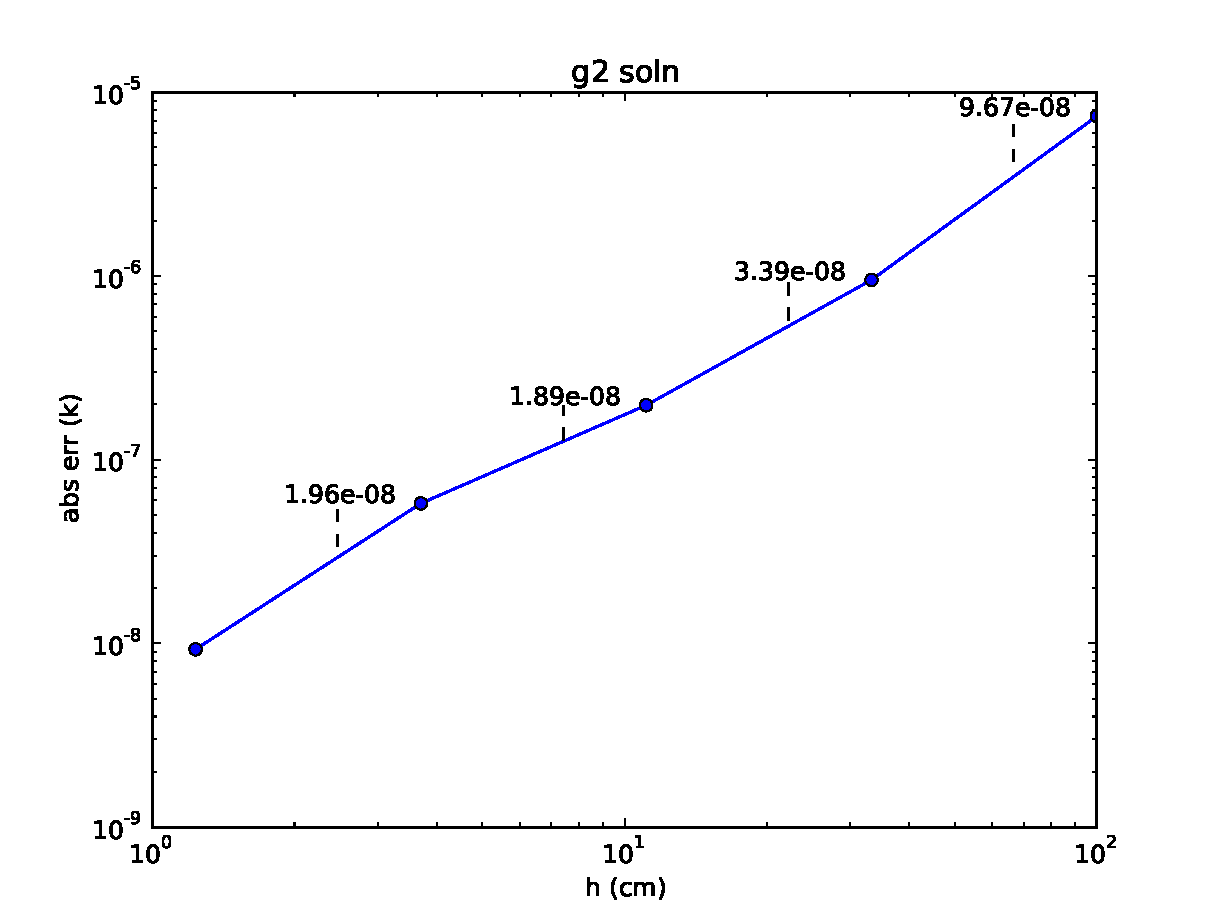
\includegraphics[width=\textwidth]{g2}
   \caption{$\phi$, Group 2}
   \label{g2}
  \end{subfigure}
  \caption{Spatial Convergence, $\phi$}
  \label{spatialphi}
\end{figure}
\begin{figure}[H]
\centering
   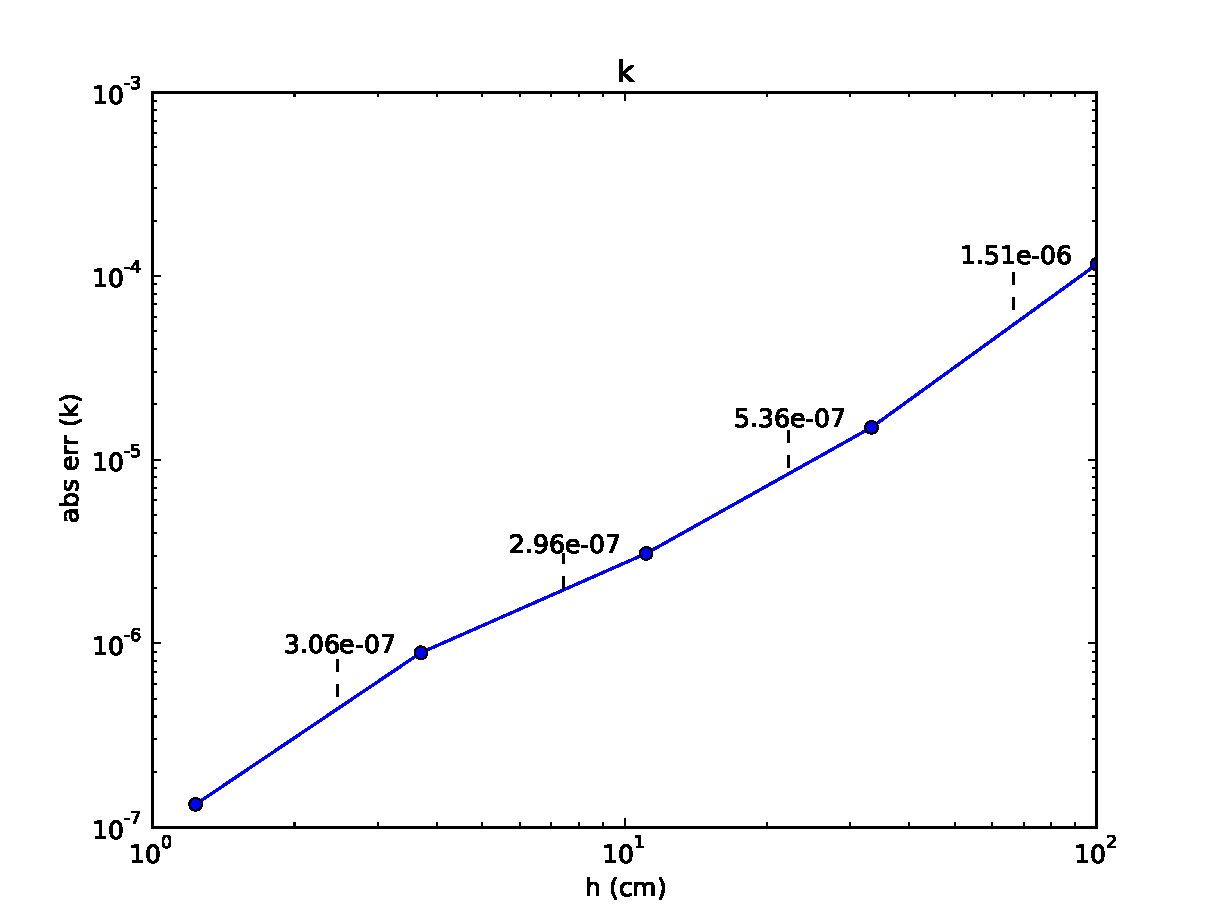
\includegraphics[width=0.5\textwidth]{k}
   \caption{Spatial Convergence, $k$}
   \label{spatialk}
\end{figure}

\subsection{Stochastic Convergence}
We consider three cases in this report, varying the number of uncertain inputs with anisotropic weights as
\begin{table}[H]
\centering
\begin{tabular}{c|c|c}
Material & Property & Distribution \\ \hline
Material 1 & $\nu\Sigma_{2,f}$ & $\mathcal{U}(0.0981,0.1201)$ \\
Material 1 & $\Sigma_{2,c}$ & $\mathcal{U}(0.0499,0.0609)$  \\
Material 4 & $\nu\Sigma_{2,f}$ & $\mathcal{U}(0.0921,0.1121)$ \\
Material 4 & $\Sigma_{2,c}$ & $\mathcal{U}(0.03732,0.04552)$  \\
Material 5 & $D_2$ & $\mathcal{U}(0.1432,0.1752)$ 
\end{tabular}
\caption{Uncertain Input Parameters}
\label{params}
\end{table}
where $\mathcal{U}(a,b)$ signifies a uniform distribution between $a$ and $b$.\\

In order for stochastic collocation to be preferable to Monte Carlo for uncertainty quantification, we desire both the magnitude of the stochastic error to be lower for stochastic collocation, and its convergence rate sufficiently fast to prevent Monte Carlo from being preferable for a given cost (number of PDE solves).  It should be noted that there does exist a difference in algorithmic computational overhead between stochastic collocation and Monte Carlo methods independent of the number of PDE solves; however, for sufficiently large numbers of solves this overhead time is insignificant compared to the overall solve time.  We consider only the number of PDE solves when considering computational cost.\\

In order to compare magnitude of error, we use a benchmark generated with a high number of collocation points using isotropic sparse grid stochastic collocation as a reference solution.  Monte Carlo and stochastic collocation solutions for varying numbers of PDE solves are computed, and relative error is plotted as a function of number of solves.  The error is in the moments $r$ of the quantity of interest $k(Y)=u(Y)$, and is given by
\begin{equation}
\epsilon_h^{(r)}=\frac{|\expv{u_h^{(r)}}-\expv{u_\text{ref}^{(r)}}|}{\expv{u_\text{ref}^{(r)}}},
%S_{N,\Lambda_\text{TD}(L)}[k_h](Y)
\end{equation}
\begin{equation}
\expv{u_h^{(r)}}=\expv{S_{N,\Lambda_\text{TD}(L)}[u_h](Y)^{(r)}}=\sum_{k=1}^\eta w_k ~u_h^{(r)}\qty(Y^{(k)}),
\end{equation}
where the weights $w_k$ and points $Y^{(k)}$ come from the multivariate quadrature used in stochastic collocation.\\

Figs. \ref{n1}-\ref{n5} show the comparison of Monte Carlo convergence to stochastic collocation for $N=1,3,5$ where $N$ is the number of uncertain parameters.  Both total degree (TD) and hyperbolic cross (HC) index sets have been included for $N>1$ (they are indistinguishable for $N=1$).  Additionally, we include two low-anisotropy anisotropic grids.\\

Because of the regularity of $k(Y)=u(Y)$, the total degree index set is as cost effective as the hyperbolic cross index set.  For a less regular stochastic solution, we expect hyperbolic cross would be more efficient.  We also expect the convergence rate to diminish with increasing $N$, and that trend can be seen in the figures for the mean and variance of $k(Y)$. Both the magnitude of the error as well as the convergence rate of stochastic collocation outperforms Monte Carlo for any number of runs.  In addition, heuristic selection of importance weighting improved the accuracy of sparse grid methods by approximately half an order of magnitude.\\
\begin{figure}[H]
\centering
  \begin{subfigure}[b]{0.49 \textwidth}
   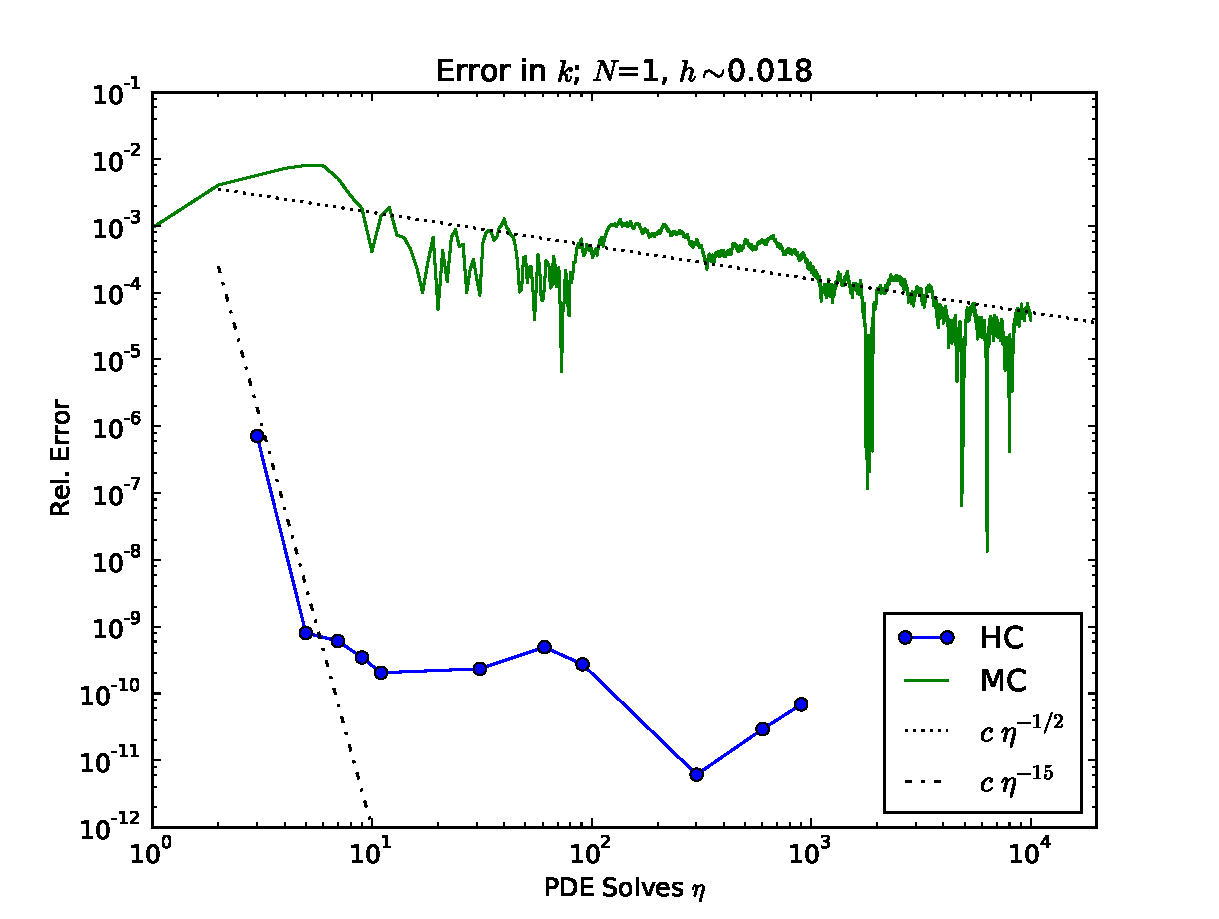
\includegraphics[width=\textwidth]{N1_h5_MCHC}
   \caption{Mean}
   \label{n1mean}
  \end{subfigure}
  \begin{subfigure}[b]{0.49 \textwidth}
   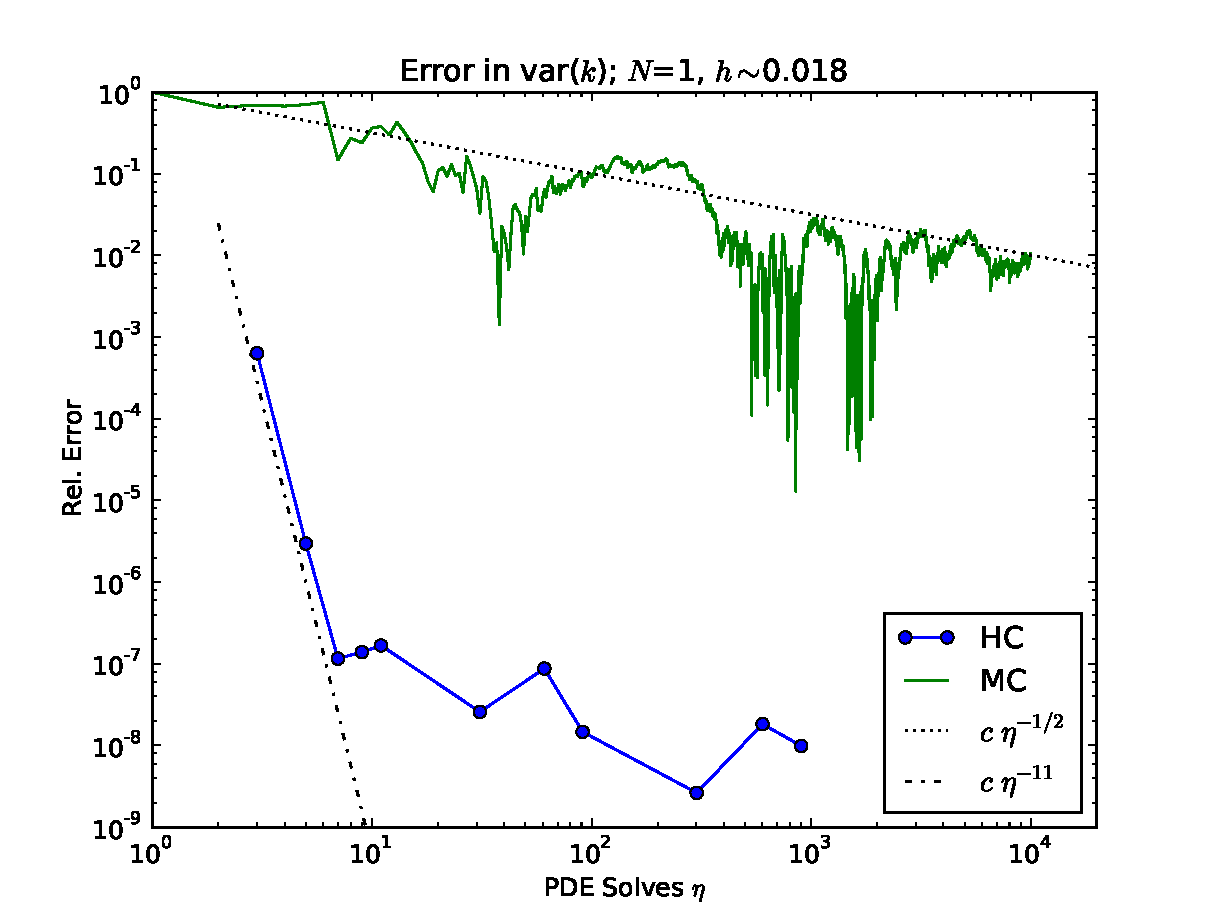
\includegraphics[width=\textwidth]{N1_h5_MCHC_2}
   \caption{Variance}
   \label{n1var}
  \end{subfigure}
  \caption{$N=1$}
  \label{n1}
\end{figure}

\begin{figure}[H]
\centering
  \begin{subfigure}[b]{0.49 \textwidth}
   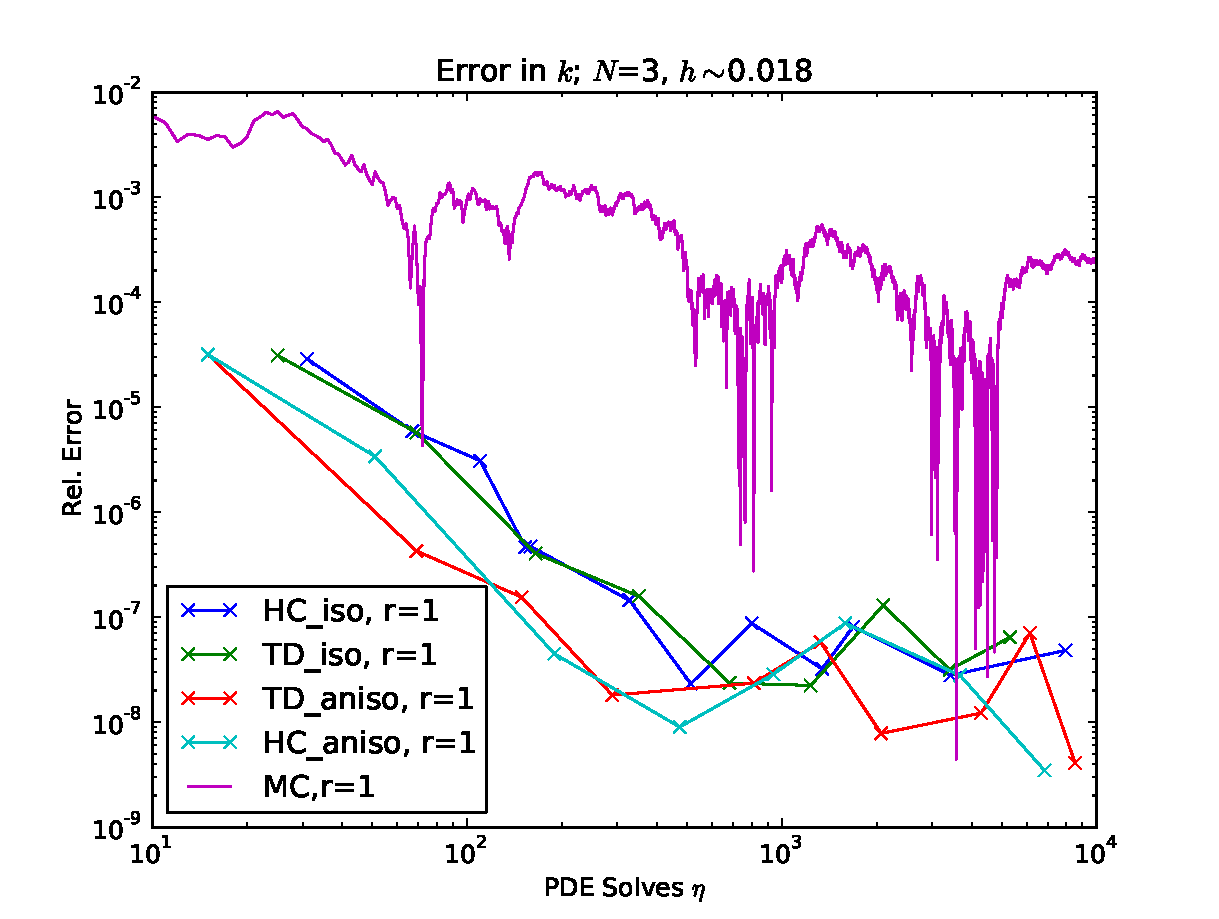
\includegraphics[width=\textwidth]{N3_h5_MCHC}
   \caption{Mean}
   \label{n3mean}
  \end{subfigure}
  \begin{subfigure}[b]{0.49 \textwidth}
   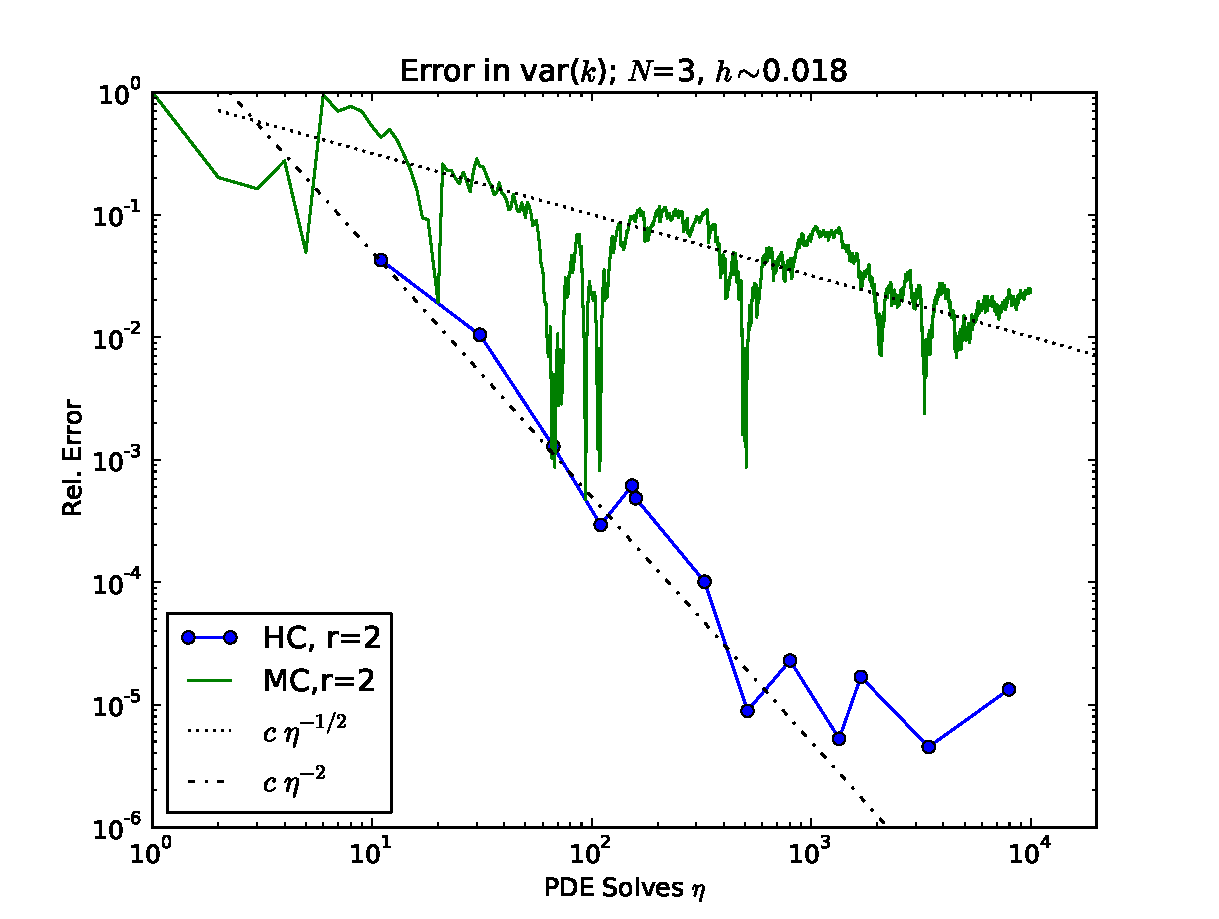
\includegraphics[width=\textwidth]{N3_h5_MCHC_2}
   \caption{Variance}
   \label{n3var}
  \end{subfigure}
  \caption{$N=3$}
  \label{n3}
\end{figure}

\begin{figure}[H]
\centering
  \begin{subfigure}[b]{0.49 \textwidth}
   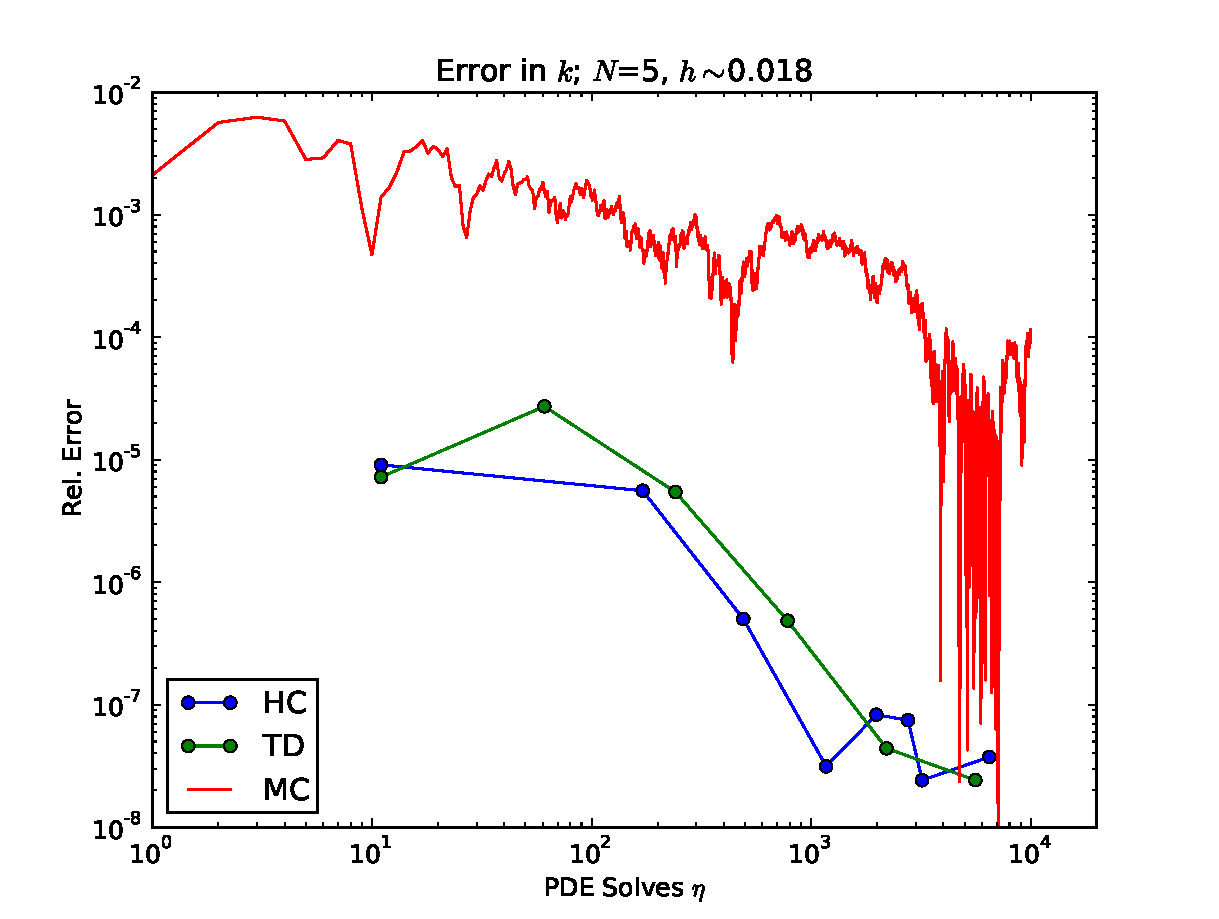
\includegraphics[width=\textwidth]{N5_h5_MCHC}
   \caption{Mean}
   \label{n5mean}
  \end{subfigure}
  \begin{subfigure}[b]{0.49 \textwidth}
   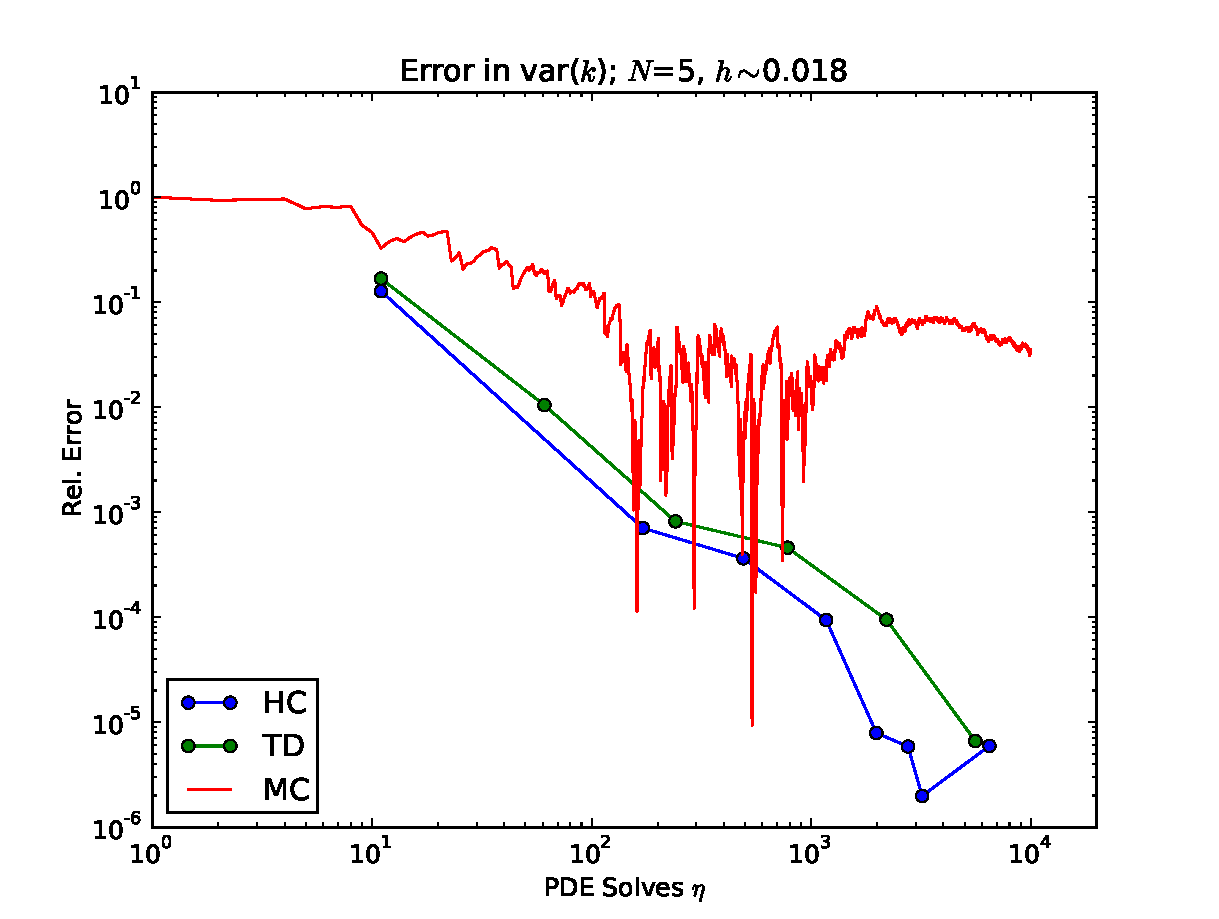
\includegraphics[width=\textwidth]{N5_h5_MCHC_2}
   \caption{Variance}
   \label{n5var}
  \end{subfigure}
  \caption{$N=5$}
  \label{n5}
\end{figure}

\subsection{Selecting Anisotropy}
Because of the heuristic nature of anisotropy importance weights, we present here several weight choices and the effect on absolute error and convergence.  We consider four cases along with Monte Carlo and isotropic sparse grids.  Each case is labeled by its importance weights in order of the input parameters listed in Table \ref{params}. The choice of weights is informed by considering the convergence rate of each individual parameter alone with increasing quadrature order, as shown in Fig. \ref{indconv}.  We surmise from this figure that the material 1 cross sections converge the slowest, while the material 5 diffusion coefficient converges most quickly.  We choose the sample cases 1-1-2-2-4 and 1-1-4-4-8 to put increasing weight on the material 1 cross sections and remove weight from the material 5 diffusion coefficient.  In addition, we choose the case 1-1-2-1-1 as an example of a somewhat arbitrary choice of coefficient to remove weight from.  Lastly, we intentionally choose a poor weighting scheme with 8-8-4-4-1 to show worst-case effects of including poor importance weights.  The results are compared in Figs. \ref{aniso1} and \ref{aniso2} for the mean and variance. 
\begin{figure}[H]
\centering
   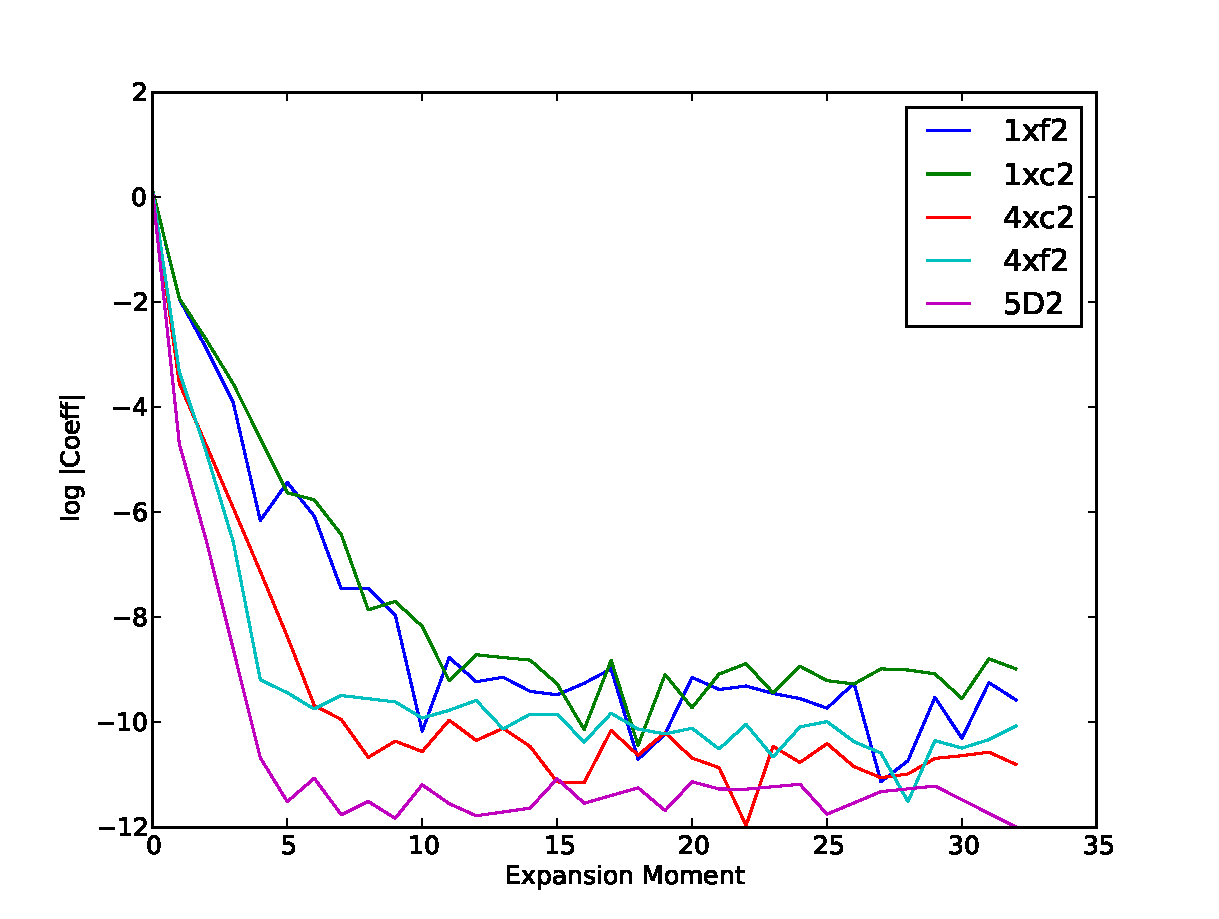
\includegraphics[width=0.5\textwidth]{coefficient_decay2}
   \caption{Independent Stochastic Convergence}
   \label{indconv}
\end{figure}
\begin{figure}[H]
\centering
  \begin{subfigure}[b]{0.49 \textwidth}
   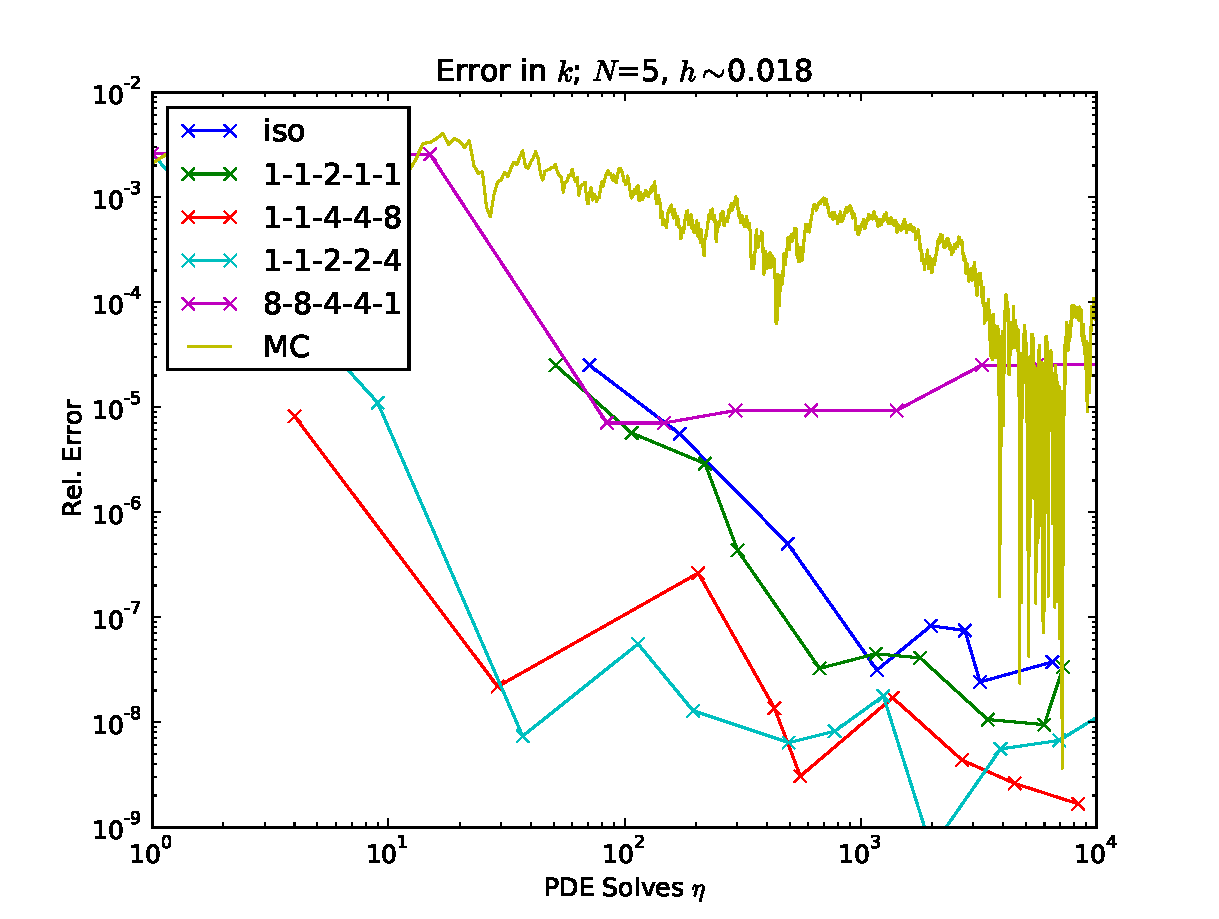
\includegraphics[width=\textwidth]{N5_h5_aniso1}
   \caption{Mean}
   \label{aniso1}
  \end{subfigure}
  \begin{subfigure}[b]{0.49 \textwidth}
   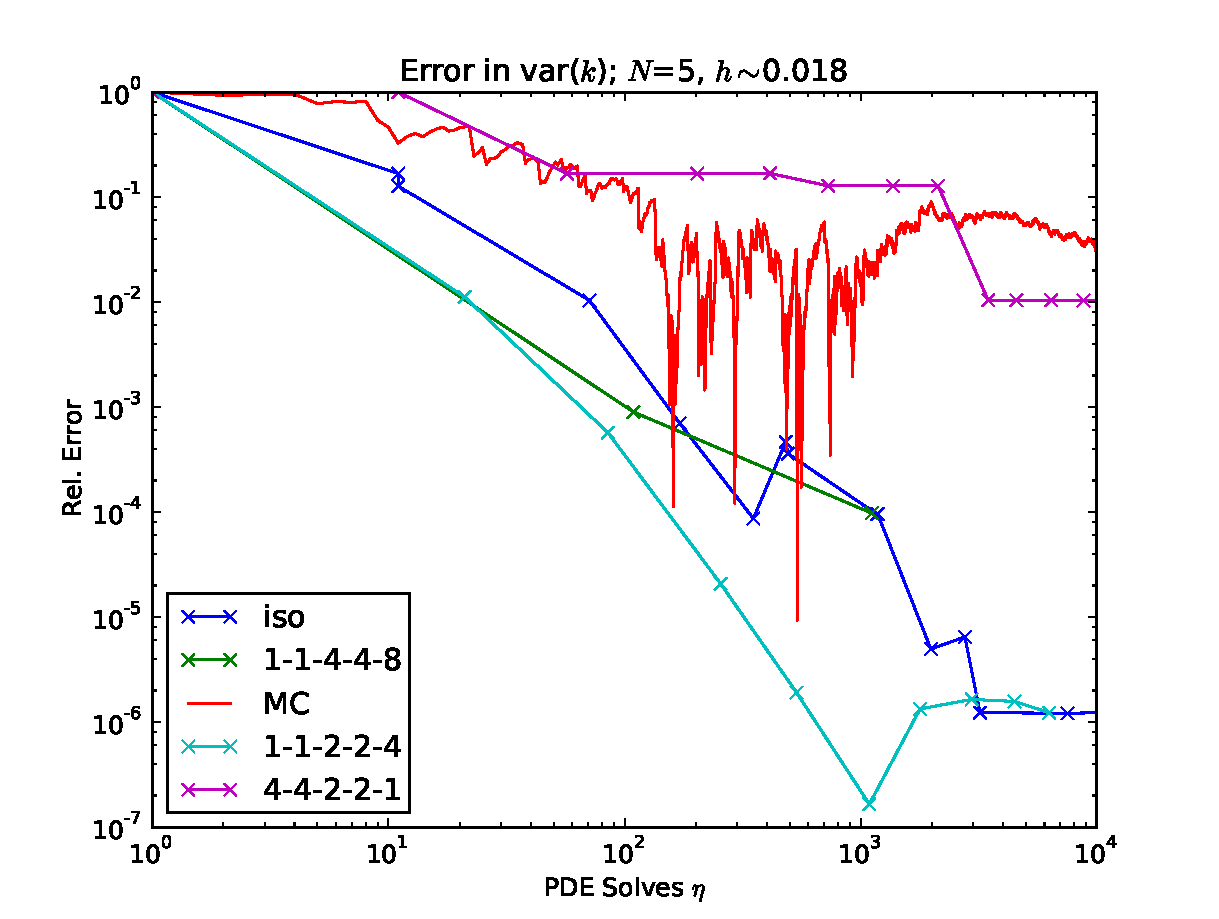
\includegraphics[width=\textwidth]{N5_h5_aniso2}
   \caption{Variance}
   \label{aniso2}
  \end{subfigure}
  \caption{$N=5$, Anisotropics}
  \label{aniso}
\end{figure}


\section{Discussion}
There are a few important considerations when analyzing Figs. \ref{n1}-\ref{aniso}.\\

First, there is a noticeable plateau in error convergence in many of the stochastic collocation plots.  Thus far this seems to be an artifact of the algorithm, originating in single-point versus double-point precision round off.  Ongoing efforts include finding any conversion of scalars from standard double precision to single precision within the algorithm.\\

Additionally, the number of PDE solves for stochastic collocation is determined based on the maximum expansion level $L$.  For higher $N$, increasing $L$ by only one value increases the number of PDE solves much more than increasing $L$ by one for small $N$.  As a result, there are few data points to power fit for $N=5$, and the plateau just mentioned around $\epsilon=10^{-8}$ is more difficult to distinguish from standard convergence.  Resolving the issues leading to the plateau should also resolve this difficulty in fitting points.  Based on trends with the variance and mean from the other plots, we expect a convergence rate of order -3 for the mean when $N=5$.\\

We can see the possible benefit and harm of applying importance weighting to an anisotropic grid in Figs. \ref{aniso}.  Any application of anisotropic sparse grids in line with our heuristic assessment significantly improves the magnitude of error for a given number of PDE solves.  Even the arbitrarily-chosen 1-1-2-1-1 shows improvements over standard isotropic HC.  We note, however, that the convergence of 1-1-2-2-4 is quite similar to 1-1-4-4-8.  This suggests that with 1-1-2-2-4 we have achieved an optimum efficiency that isn't improved with further anisotropy.  However, the anisotropy intentionally chosen poorly shows much worse convergence than the isotropic case, and for the variance is on par with Monte Carlo.\\

Given these limitations, it is clear that for the uncertain spaces presented, stochastic collocation shows much better convergence and magnitude of error for the same cost when compared with Monte Carlo.  In addition, using judgement to apply an importance weight to variables yields additional rewards in efficiency.

\section{Ongoing Work}
The work presented here considers a maximum number of uncertain variables $N=5$.  While demonstrative of expected savings for larger input spaces, showing the convergence rates of isotropic and anisotropic sparse grids for large $N$ is desirable.  We expect to see diminishing returns in using stochastic collocation as the input space grows in dimensionality.\\

One effective method for very large numbers of uncertain inputs is HDMR, which uses sets of low-order stochastic interactions between a few variables at a time to approximate the full stochastic problem.  In the event the number of uncertain parameters becomes very large, HDMR could prove less costly than stochastic collocation for many problems. \\

Lastly, our work so far has been demonstrated exclusively with uniformly-distributed random variables as input parameters.  To more accurately approximate the shape of an arbitrary probability distribution, we intend to implement Beta-distributed random variables using Jacobi quadrature, with two shaping parameters $\alpha,\beta$.  The Beta distribution is also distributed finitely between two points, but $\alpha,\beta$ can be adjusted to accommodate a wide range of uncertain distributions including uniform and truncated Gaussian normal distributions.  While Beta distributions cannot exactly replicate all other distributions, we expect it can replicate them without introducing a greater error than introduced by the Monte Carlo and stochastic collocation methods presented.

\newpage
\bibliography{uq}{}
\bibliographystyle{plain}
\end{document}